\documentclass[final, 3p, 11pt]{elsarticle}

% Packages
\usepackage{lmodern}
\usepackage[T1]{fontenc}
\usepackage{amsmath}
\usepackage{graphicx}
\usepackage{booktabs}
\usepackage{multicol}
\usepackage[version=4]{mhchem}
\usepackage{subcaption}
\usepackage{listings} % For code
\usepackage{float}

\usepackage[numbers]{natbib}
\bibliographystyle{unsrtnat}

\setlength{\parskip}{1em}
\setlength{\parindent}{0pt}

\makeatletter
\def\ps@pprintTitle{%
 \let\@oddfoot\@empty
 \let\@evenfoot\@empty
}
\makeatother

% Python code style settings
\lstset{
  basicstyle=\ttfamily\footnotesize,  % Code font
  numbers=left,                       % Line numbers
  numberstyle=\tiny,                  % Line number style
  numbersep=5pt,                      % Line number spacing
  language=Python,                    % Python syntax highlighting
}

\usepackage[hidelinks]{hyperref}

% Begin document
\begin{document}
\begin{frontmatter}

% Title Page

\title{4TR3 - Capstone Midterm Report\\}
\title{Non-intrusive Testing of Liquid Culture Medium using Online NIR Spectroscopy and Machine Learning for Qualitative Analysis}

\author[1]{Benjamin Samuel - studentID \fnref{cor3}}
\author[1]{\\Connor Reintjes - studentID \fnref{cor1,cor2}}
\author[1]{\\Paola Gonz\'alez P\'erez - studentID \fnref{cor2}}
\author[1]{\\Shiza Hassan - studentID \fnref{cor3}}
\author[1]{\\Dr. Amin Reza Rajabzadeh\fnref{cor4}} % Supervisor as corref

\fntext[cor1]{Conceptualization} % Custom footnote for dry-lab-1
\fntext[cor2]{Validation \& Software} % Custom footnote for dry-lab-2
\fntext[cor3]{Investigation \& Methodology} % Custom footnote for wet-lab
\fntext[cor4]{Principle Investigator \& Capstone Supervisor} % Custom text for Supervisor

\affiliation[1]{organization={McMaster University, W. Booth School of Engineering Practice and Technology}, city={Hamilton, ON.}, country={Canada}}

\begin{abstract}
Insufficient quality assurance is a major expense associated with laboratories that an result in contamination, poor sample integrity, and lead to lost time due to repetitive sample testing. To ameliorate these issues, NIR spectroscopy has been combined with machine learning in this approach to qualitatively analyze the composition of liquid cultures in a non-intrusive and online manner. This will allow laboratories to save time by identifying contamination as soon as it happens and proceeding accordingly, as opposed to finding out after a full protocol has been performed. The method to achieve this involved creating a handheld casing to house the NIR which would take spectra of the sample and pass it to a machine learning model that would then identify whether the sample is in a normal or contaminated state. In phase 1 of the experiment, the NIR housing was manufactured and initial testing was conducted for both contaminated and non-contaminated states, with the contaminant being \textit{Lactobacillus rhamnosus}. The results achieved indicate that the NIR was able to differentiate between contaminated and non-contaminated samples. In phase 2, further data collection was conducted using a quartz cuvette and Teflon background to reduce noise and spectra interference. A data augmentation pipeline was constructed to overcome data size limitations. The processed data was then fed into a 1D-CNN model to obtain preliminary results on its performance. Implementation of one-class classification resulted in the overfitting of the model. The pipeline and 1D-CNN model will continue to be developed in order to improve their performance as more diverse data is collected.

\end{abstract}

\begin{keyword}
Bioprocess Monitoring \sep Machine Learning \sep Near Infared Spectroscopy (NIR) \sep 1D Convolutional Neural Network (1D-CNN) \sep Qualitative Analysis
\end{keyword}

\end{frontmatter}

% Introduction

\section{Materials and Methods}

\subsection{\textit{L. Rhamnosus} Viability Test}
The \textit{Lactobacillus rhamnosus} viability test was conducted at the beginning of the term before running the experiments to ensure that the bacteria were alive when it came time to test the contaminated samples. This was performed by initially sterilizing the environment by lighting a Bunsen burner on an absorption mat. Then four MRS agar plates were inoculated with bacteria from the frozen samples from the previous term using an inoculating loop. Two samples each were taken from the hyperconcentrated and normal concentration samples, and one MRS plate was left untouched to serve as the control. The cells were evenly spread throughout the plate using a cell spreader to ensure even growth and the plates were then closed and wrapped with parafilm. They were then incubated at 37°C for 24 hours to allow for the bacteria to grow. 

\subsection{NIR Housing Design}
The custom housing for the NIR was 3D printed using a Bambu Lab P1S. The majority of the housing was constructed using Acrylonitrile butadiene (ABS) filament however, the cuvette holder was printed using polylactic acid (PLA) filament. The sides and bottom of the cuvette holder were printed in black PLA, while the background was printed in white PLA to increase reflectance. 

This white PLA background was not as reflective as originally theorized, so the use of teflon (PTFE) was considered. A high-reflectance PTFE sheet with 3M Adhesive backing was purchased from ThorLabs. This sheet has a reflectance $( >90\%)$ in the UV spectrum, and is one factor attributed to improving the signal-noise-ratio (SNR) within the scans \citep{HighReflectancePTFESheets}.

\subsection{Cuvette Material}
As noted in the previous term, the plastic cuvettes were giving an unclear result with noise, and in comparison, the quartz cuvette offered a much clearer result. As a result, the quartz cuvette was used instead and there was a subsequent improvement in the clarity of the results. With the change from plastic to quartz cuvette, the time taken to set up the run was comparatively longer. Plastic cuvettes were disposed of at the end of each run and a new cuvette was used to set up the consequent runs. However, with the quartz cuvette, the cuvette with the fermented broth was first rinsed with bleach and safely disposed of in liquid waste containers. It was then rinsed with DI water and then ethanol. Finally, it was rinsed with methanol and then dried using a vacuum pump. This ensured that the quartz cuvette was properly cleaned before the next run, thereby allowing for scans that did not have any interference or contamination.

\subsection{Data Augmentation}
Due to the limited number of samples that were able to be collected, the data was augmented for the sake of training. Different data augmentation methods were explored to best fit our use case. Factors such as simplicity, and reducing the risks of overfitting were considered. The use of subsampling was determined to be the optimal method and was applied to future data collection.

\subsubsection{Pipeline Subsampling}
The data augmentation pipeline that was created is based on a type of subsampling called cyclic subsampling. Cyclic subsampling divides the dataset into non-overlapping subsets using an offset starting index and a set interval. This method has a few key features that make it optimal for this dataset when compared to other methods like temporal subsampling with sliding windows or random sampling. Since the interval remains the same across all subsamples, the temporal order of the dataset can be maintained when training a neural network. The non-overlapping sub-samples have a lower redundancy within the datasets compared to other methods, which will help prevent overfitting. The improved diversity would also allow the model to account for variations in starting time or time accumulation from scan duration.

\subsubsection{Subsampling Considerations}
Using cyclic subsampling had some major considerations that changed future data collection. The subsample interval would have to be large enough to prevent redundancy, while also remaining small enough to not create a large margin of error within the model. The frequency of scans would also have to be high enough to prevent the offset time points from approaching the cycle interval. Due to these considerations, our scanning frequency was changed to 60 second intervals. Our default augmentation parameters were set at a 60 second offset with a 15 minute (900 second) cycle interval with 3 subsamples per dataset.

\subsection{Data Processing}
In addition to subsampling the data, the samples underwent additional processing. The only processing step originally implemented was scaling/normalization. The Scikit Learn processing package “MinMaxScalar” was used to perform this step. According to the scikit-learn API reference documentation, the purpose of the MinMaxScalar is:
\begin{quote}
This transformation is often used as an alternative to zero mean, unit variance scaling. MinMaxScaler doesn’t reduce the effect of outliers, but it linearly scales them down into a fixed range, where the largest occurring data point corresponds to the maximum value and the smallest one corresponds to the minimum value \citep{ScikitLearnAPI}.
\end{quote}
The purpose of this processing step is to scale all of the data between 0 and 1 in order to better observe the key features within the same range. It uses the formula found in \autoref{eq:minmax}.

\begin{equation}
X_{\text{scaled}} = \frac{X - X_{\text{min}}}{X_{\text{max}} - X_{\text{min}}} \times (f_{\text{max}} - f_{\text{min}}) + f_{\text{min}}
\label{eq:minmax}
\end{equation}

\subsection{One-Dimensional Convolutional Neural Network}
The classification of near-infrared (NIR) spectra to determine the contamination state of liquid media was performed with a one-dimensional convolutional neural network (1D-CNN). This neural network model uses the Keras library with Tensorflow as the backend. The use of Keras facilitates the modelling of the CNN due to its intuitive and user-friendly interface \citep{kerasteam_keras}. The Tensorflow backend allows for accelerated training when used with GPU \cite{acecloudteam_2024_tensorflow}. It also enables a detailed visualization through Tensorboard. Their combination results in a flexible model with easily customizable variables, like the layers and optimizers, along with shorter training times

\subsubsection{Model Architecture}
The model consists of two Conv1D layers, with 64 and 32 filters respectively. These filters allow for the extraction of significant features in the input data \citep{nisha_2020_applications}. These features set the parameters that will be learned throughout training. To avoid overfitting and reduce the dimensionality of these parameters, MazPooling1D layers and Dropout layers are implemented after the Conv1D layers. The activation function, or function that transforms the input of a node into an output of that node, is a key component of a neural network. The model uses the Rectified Linear Unit (ReLU) function as the activation function, which only outputs non-negative outputs or zeros (Brownlee, 2019). This is commonly used in CNNs due to its ease of training and superior performance. A final dense layer is implemented with a sigmoidal activation function. This function outputs a probability score between 0 and 1 to determine the contamination state of the sample: 0 for non-contaminated and 1 for contaminated \citep{saeed_2021_a}.

\subsubsection{Optimizer and Loss Function}
Optimizers are functions responsible for adjusting the parameters as training progresses \citep{eitcaacademy_2023_what}. This is done to reduce the loss function, a mathematical quantification of the error margin between the prediction and the ground truth. The Adam algorithm was chosen as the optimizer. This follows a stochastic gradient descent based on adaptive estimation and regulated by the learning rate \citep{kerasteam_keras}. It allows for the model to reach an optimal point faster without taking large learning steps that could lead to skipping key information during training. The learning rate was set to 0.0005 to avoid reaching a convergence between the ground truth and prediction too early during training.

\begin{equation}
    L = -\frac{1}{N} \sum_{i=1}^{N} \left[y_i \cdot \log(p(y_i)) + (1 - y_i) \cdot \log(1 - p(y_i)) \right]
  \label{eq:cross_entropy}
\end{equation}

The binary cross-entropy loss function was used in the model due to the binary classification nature of the project. This loss function is defined as where y is the label (1 for contaminated and 0 for non-contaminated) and $p(y)$ is the predicted probability of the point being contaminated for all N points. Binary cross-entropy quantifies the differences between the logarithmic probability distributions and penalizes inaccurate predictions which helps assess the model’s prediction confidence.

\subsubsection{Training Parameters}
Since the small size of the training dataset represents a major problem for the accuracy of the model, the number of epochs, or cycles that the entire dataset passes through the algorithm during training, was adjusted to offset this limitation. The model was trained with 15 epochs to reduce the risk of overfitting, and an early stopping callback was included to stop the training process once the model showed no further improvement after each epoch. To ensure an efficient use of the limited dataset for both training and validation, cross-validation was implemented. This allowed for both the training and validation batch size to be 18, the total dataset size.

\subsubsection{One-Class Training}
he imbalanced data classes caused by the lack of data on contaminated samples resulted in the need to implement one-class training on the non-contaminated samples. This approach is commonly known as one-class classification or unary classification \citep{brownlee_2020_oneclass}. It enables the model to learn the characteristics of the “normal”, in this case, the non-contaminated samples, and subsequently classify between this data type and deviation from it, such as contaminated samples.

\subsubsection{K-Fold Cross Validation}
To maximize the use of the limited data in both training and validation, as well as provide a more robust model evaluation, cross-validation was implemented with the K-fold method. This consists of splitting the dataset into k folds and using each fold once as a validation set while using the other folds for training. Due to the small dataset, the k was set to be 3 to maintain the same ratio of data per fold and maintain a balanced class distribution.

\subsubsection{Visualization of Metrics}
To permit an easy understanding of the model’s performance, the primary training metrics were visualized using TensorBoard. The loss, accuracy, and learning rate changes were tracked in real-time during the training phase. These metrics were used to produce four plots: (\autoref{fig:all_fold_acc}) combined validation loss and accuracy over epochs for all folds, (\autoref{fig:per_fold_acc}) validation accuracy per fold, (\autoref{fig:conf_matrix}) confusion matrix, and (\autoref{fig:roc_curve}) receiver operating characteristic (ROC) curve. The validation loss and accuracy over the epochs plot show the progression of the training as the number of epochs increases. The validation loss indicates how effectively the model is learning allows to observe if overfitting or underfitting of the model is occurring. The validation accuracy indicates how well is the model improving its prediction accuracy during the training phase. Including these two metrics for the different folds in the same plot allows for a clear comparison of the improvement of the model as the cross-validation fold increases. The confusion matrix provides a detailed and intuitive visualization of the model’s prediction performance \citep{hernndezdeltoro_2022_assessing}. It compares the ground truth labels against the predicted labels of the test data, showing the counts for true positives, true negatives, false positives, and false negatives. The ROC curve shows the classifier performance across different thresholds \citep{googlefordevelopers_2024_classification}. It requires calculating the true positive rate and the false positive rate at each threshold to plot these together. The resulting area under the curve represents the probability that the model can properly classify between classes. An area under the curve equal to 1.0 represents a perfect model with low random classification. These plots provide an overview of the model performance and allow for the assessment of the training process to identify potential overfitting.

 
\section{Results}

\subsection{\textit{L. Rhamnosus} Viability}
The results of the lactobacillus viability test as seen in \autoref{fig:bacteria_viability} (from left to right) showing the control plate, hyperconcentrated sample, and normally concentrated sample with their respective growths. The second row shows the replicate that was created for the hyperconcentrated and normal samples to ensure reproducibility of the results.

\subsection{Ethanol Curves}
To analyze the results of the graphs (\autoref{fig:appendix_ethanol_plastic} \& \autoref{fig:appendix_ethanol_standard}), the second overtone of the \ce{C-H} stretching vibration, just before $1200\text{nm}$, is considered. This overtone is representative of ethanol as it indicates the pronounced symmetrical vibration of the methyl group.

A detailed analysis of the results from experiments that were previously carried out revealed that the peaks observed from the NIR spectrophotometer were not sufficiently distinct to accurately identify the presence of ethanol. To improve the accuracy of the CNN model, and ensure that the data is reliable, the peaks had to be observed with less noise and be clearly distinct. The use of plastic cuvettes was identified as a factor that contributed to the suboptimal peak resolution. This issue was addressed by replacing the plastic cuvette with a quartz cuvette for data collection runs. 
Quartz cuvettes are highly durable and resistant to scratches, thereby being an ideal material to run experiments frequently whereas plastic cuvettes had to be discarded after a single-use \citep{CuvettesSpectrophotometerComprehensive2023}. Moreover, quartz has the least path length variation when compared to alternate materials like glass and plastic, ensuring that the results collected were consistent and reproducible. Another key advantage is quartz’s ability to withstand high temperatures, which is essential for extended NIR spectroscopy experiments. Since scans were taken every minute for 24 to 48 hours, the spectrometer generated significant heat, and quartz cuvettes could endure these conditions without compromising performance. On the other hand, the quartz cuvette did have a high initial cost. Since the benefits outweigh the drawbacks, the quartz cuvette was our choice of material to replace plastic.

Teflon tape was applied to the housing of the spectrometer to improve the quality of NIR spectroscopy measurements and minimize noise. Placing the tape at the rear of the cuvette absorbed stray light rays that would otherwise cause scattering and distortion, thus improving the precision of the absorbance readings. This adjustment reduces interference and ensures a more stable light pathway, allowing the spectrometer to capture a broader and more consistent range of absorbance values. 

The resulting absorbance curves exhibit smoother transitions, with well-defined dips that reflect the dynamics of the yeast fermentation process more clearly, free from erratic fluctuations. The gradual slopes and smooth dips contribute to a more refined and optimal spectral output, enabling subtle variations in ethanol production to be more accurately detected. This improvement in the clarity and aesthetics of the spectral curves enhances both the interpretability and the visual appeal of the scans, ultimately supporting more precise data analysis.

\subsection{Model Training and Validation}
The validation accuracy for all folds, observed in \autoref{fig:all_fold_acc}, remains constant across all epochs, with a value of 1.0. On the other hand, the validation fold for each fold shows a constant decrease as the epoch number increases. The loss values at the start of the training for each fold are relatively high. These then show a steady decline, approaching near-zero values by the final epochs. Fold 1 shows the highest initial loss compared to the other folds, but the decreasing trend remains similar across folds. This steady decrease indicates the model’s success in minimizing the loss during training.

\begin{figure}
        \centering
        \begin{subfigure}[b]{0.505\textwidth}
            \centering
            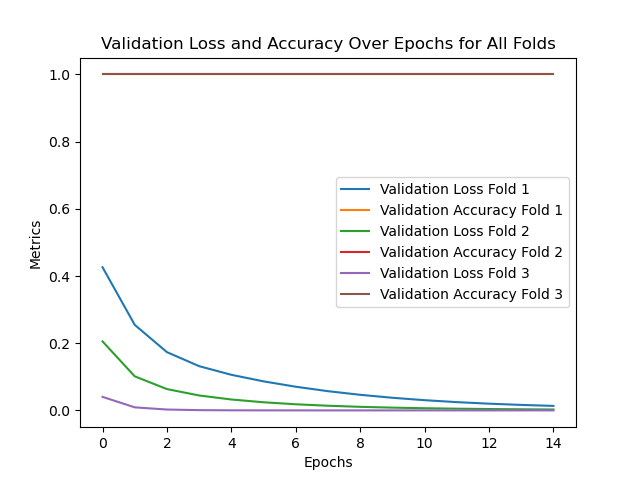
\includegraphics[width=\textwidth]{Images/validation_loss.png}  % Replace with your image file
            \caption{All Fold Validation Loss and Accuracy}
            \label{fig:all_fold_acc}
        \end{subfigure}
        \hfill
        \begin{subfigure}[b]{0.485\textwidth}
            \centering
            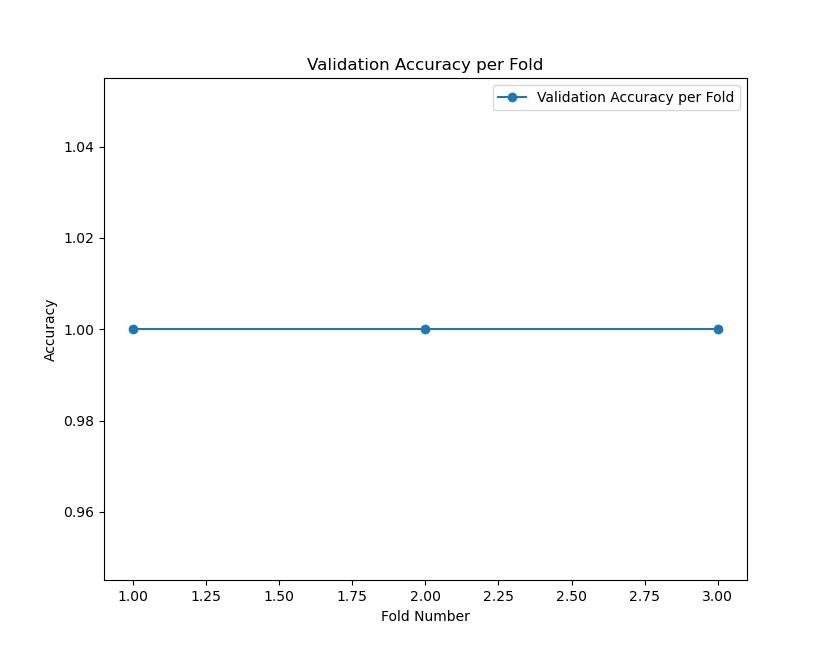
\includegraphics[width=\textwidth]{Images/validation_accuracy.png}  % Replace with your image file
            \caption{Per Fold Validation Accuracy}
            \label{fig:per_fold_acc}
        \end{subfigure}
        \caption{Model Accuracy and Validation from Preliminary Training}
        \label{fig:model_accurary}
    \end{figure}

The final validation accuracy achieved per fold, shown in \autoref{fig:per_fold_acc}, shows that each of the three folds achieved an accuracy of 1.0. The static accuracy across all folds often represents a model that consistently performs at a high level during cross-validation. However, the observed consistency may be misleading, as it also relates to the overfitting of small and imbalanced datasets.


\begin{figure}
        \centering
        \begin{subfigure}[b]{0.53\textwidth}
            \centering
            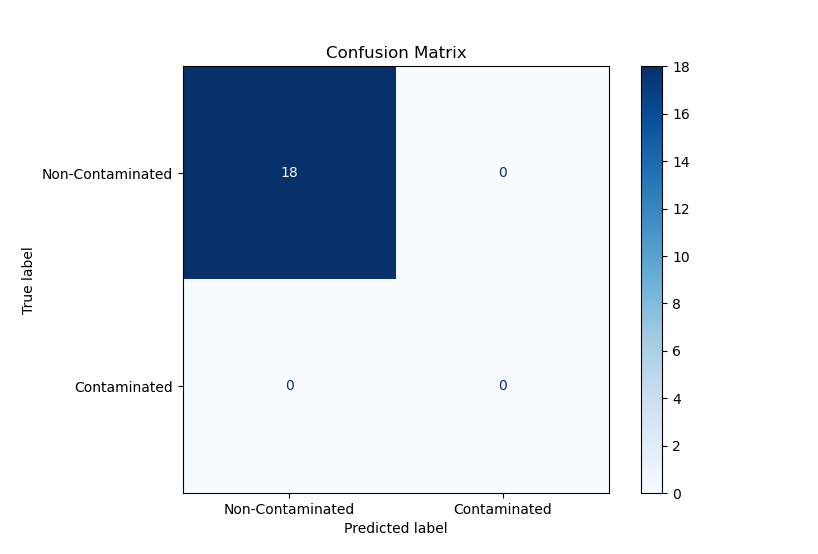
\includegraphics[width=\textwidth]{Images/confusion_matrix.png}  % Replace with your image file
            \caption{Model Confusion Matrix}
            \label{fig:conf_matrix}
        \end{subfigure}
        \hfill
        \begin{subfigure}[b]{0.46\textwidth}
            \centering
            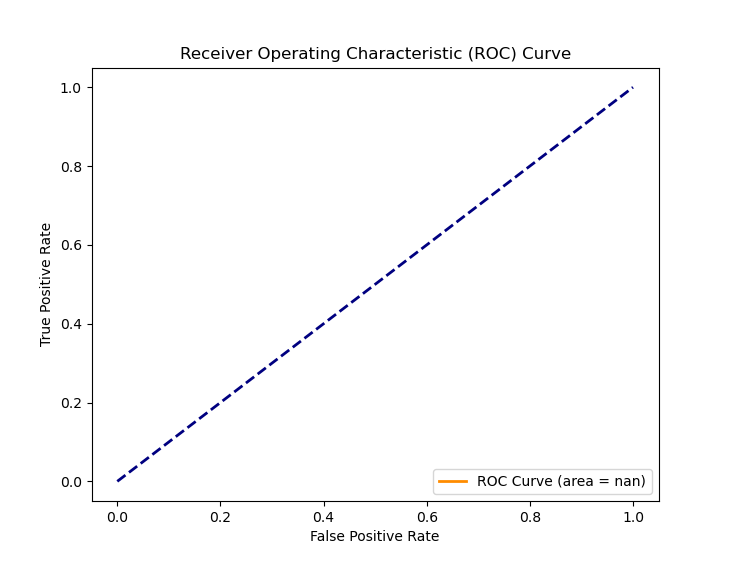
\includegraphics[width=\textwidth]{Images/roc_curve.png}  % Replace with your image file
            \caption{Receiver Operating Characteristics Curve}
            \label{fig:roc_curve}
        \end{subfigure}
        \caption{Model Validation Testing}
        \label{fig:matrix_roc}
    \end{figure}

The confusion matrix (\autoref{fig:conf_matrix})shows the ability of the model to correctly classify the 18 non-contaminated samples. However, the model fails to classify contaminated samples, indicating a bias towards the larger class as it has not learned to identify other data classes. The biased training and prediction further support the overfitting of the model during training.

The ROC curve, observed in \autoref{fig:roc_curve}, shows a diagonal line from (0,0) to (1,1) and an area under the curve of not a number (NaN). This indicates that the model’s ability to differentiate between classes is random guessing, with a $50\%$ probability of correctly ranking the ground truth. Hence, this trend visually represents the lack of meaningful learning of discriminatory features due to the lack of diverse data. 

\section{Discussion}

The results of the \textit{Lactobacillus rhamnosus} viability test indicate that the bacteria is alive as it was able to grow on the MRS agar plate. This can be seen through the growth observed on the plates in \autoref{fig:bacteria_viability} post-incubation compared to the control plate which showed no growth. Due to the plates being left in the incubator for longer than 24 hours, the sample appeared dry when it was being taken out, however, based on the physical appearance compared to the control, it is clear the bacteria was able to grow. The hyperconcentrated samples showed more growth compared to the normal concentration, likely as a result of the increased bacteria. Based on the results of this test, contaminated runs can be performed and should give similar readings as those seen in the previous term. 
Over the course of the term, certain issues have been noted with the NIR’s data collection. The protocol that was initially being used involved collecting results over the course of 48 hours to monitor the changes in ethanol production. Unfortunately, there were issues with the laptop that would cause it to not be able to take scans for the full 48 hours, and instead stop collecting results earlier. As a result, we had an abundance of results in the first 0-24 hour range and decided to change the protocol to focus on the first 24 hours instead. To increase the dataset, data augmentation techniques were employed and will continue to be employed for the remaining runs. 

Another recent issue that has been encountered was a spill that occurred in the NIR that led to changes in the results. The NIR housing was found knocked over and the fermentation sample that was inside spilled all over the contents of the NIR and housing. After cleaning the contents and wiping down the NIR with ethanol, the unit was tested using varying concentrations of ethanol to determine if it was still reporting results similar to what was observed thus far. After doing so, there was a noticeable difference in the results, however, this is being investigated and normalization or scalability techniques may be applied to correct the data. 

High validation accuracy in this case suggests overfitting of the model due to the accuracy remaining at a constant value of 1 as the epochs increase. The limited number of training samples, each with little variation, is causing the model to “memorize” the individual samples instead of recognizing the general features of the dataset. This will drastically limit its effectiveness in classifying new or future datasets. Currently, the model is only able to be trained on one class of data, which is the non-contaminated sample. This also leads to overfitting due to the lack of diversity which will limit its ability to discriminate important features. The confusion matrix highlights the need to include representation of other classes during the training and validation of the model, as well as maintaining a balance between the dataset classes. 

\section{Problems and Future Steps}
For the continuation of the project, four main activities are proposed to ameliorate the model’s performance: verification of the NIR’s proper functioning, further non-contaminated and contaminated data collection, additional data augmentation, and model re-training. 

UV/Vis spectroscopy will be used to measure the levels of biomass. Measurements will be done at the start and at the end of the experiment. This change in absorbance reading would show the accumulation of biomass. The wavelengths to be used in recording the absorbance values are $550$, $600$, and $700\text{nm}$. Theoretically, the final absorbance readings at the end of the fermentation process, at the 24-hour mark or after, should differ from the preliminary absorbance values. This would represent microbial growth with successful fermentation. Coupling NIR and UV/Vis spectroscopy conducts a comprehensive course of fermentation, hence improving the reliability and reproducibility of the results.

The current use of strategies like single-class training, Stratified K-Fold cross-validation, and model checkpoints was based on the need to use the limited data set as efficiently as possible for both training and validation of the model. While the augmentation of the data resulted beneficial to triplicate the dataset from the original data collected, the model performance results indicate the need to increase the training and validation batch. The current model will be further refined once more data from the non-contaminated samples is obtained, and when contaminated data becomes available. A balanced contaminated and non-contaminated data set will allow for a comprehensive multi-class training model capable of a more accurate classification. Moreover, data augmentation techniques to synthetically expand the dataset will be further explored to overcome the limitations of the project. Transformations such as Gaussian noise and random sampling could improve the model’s robustness by increasing the dataset size.

The addition of algorithms like Gaussian Noise could help to improve the model further in a few areas. The addition of noise in the dataset will improve variation which can help to prevent overfitting of the model \citep{yeImprovingMachineLearning2023}. Noise will have to be tested and implemented carefully, as it can cause problems if done incorrectly. Higher instability of training, longer convergence and non-realistic data are some of the major concerns with improper implementation of noise into the dataset \citep{kuskEffectGaussianNoise2023}.


\section{Conclusion}
NIR spectroscopy was optimized to monitor ethanol production in yeast fermentation by addressing initial challenges with sharpness and noise in the absorbance curves. Quartz cuvettes replaced plastic ones to enhance light transmission and minimize interference. Additionally, Teflon tape was applied to the spectrometer housing, reducing stray light and smoothing out sharp peaks, resulting in cleaner and more stable spectral curves. Implementing these changes allowed for optimal scans that allowed for the accurate training of the machine learning model. Furthermore, the clarity of the spectral curves allows for easier interpretability of the results.

The data processing pipeline was effective at compiling the raw data,  running it through basic normalization and scaling calculations, and exporting it for model training. However, the pipeline will have to be adjusted in future to adapt the processed data to better fit the needs of training such as adding Gaussian noise. Although the model is currently able to reduce the validation loss, the high static validation accuracy across all folds, the confusion matrix results, and the ROC curve strongly support that the model is overfitting as a result of the limited data. Future improvements will focus on expanding the dataset, incorporating multiple classes, and applying regularization techniques to reduce overfitting. The actions taken thus far have improved the clarity of the results, such as the quartz cuvette, and focusing on the first 24 hours of data collection instead of 48 hours. Some issues that were encountered over the course of the semester include problems with the data collection as well as the spill in the NIR which will require further testing to ensure the NIR is still producing the expected results. Solutions to these problems are currently being employed or will be over the next few weeks. 

\newpage
\bibliography{references}     % The .bib file name (without the .bib extension)

\newpage
% \section*{Appendix}

\section*{Appendix A}

% Change the figure labeling format for this appendix
\renewcommand{\thefigure}{A.\arabic{figure}}
\setcounter{figure}{0}  % Reset the figure counter

\begin{figure}[H]
    \captionsetup{justification=raggedright, singlelinecheck=false, position=above}  % Caption on top and left-justified
    \caption{\textit{L. Rhamnosus} Viability on MRS plates.}
    \centering
    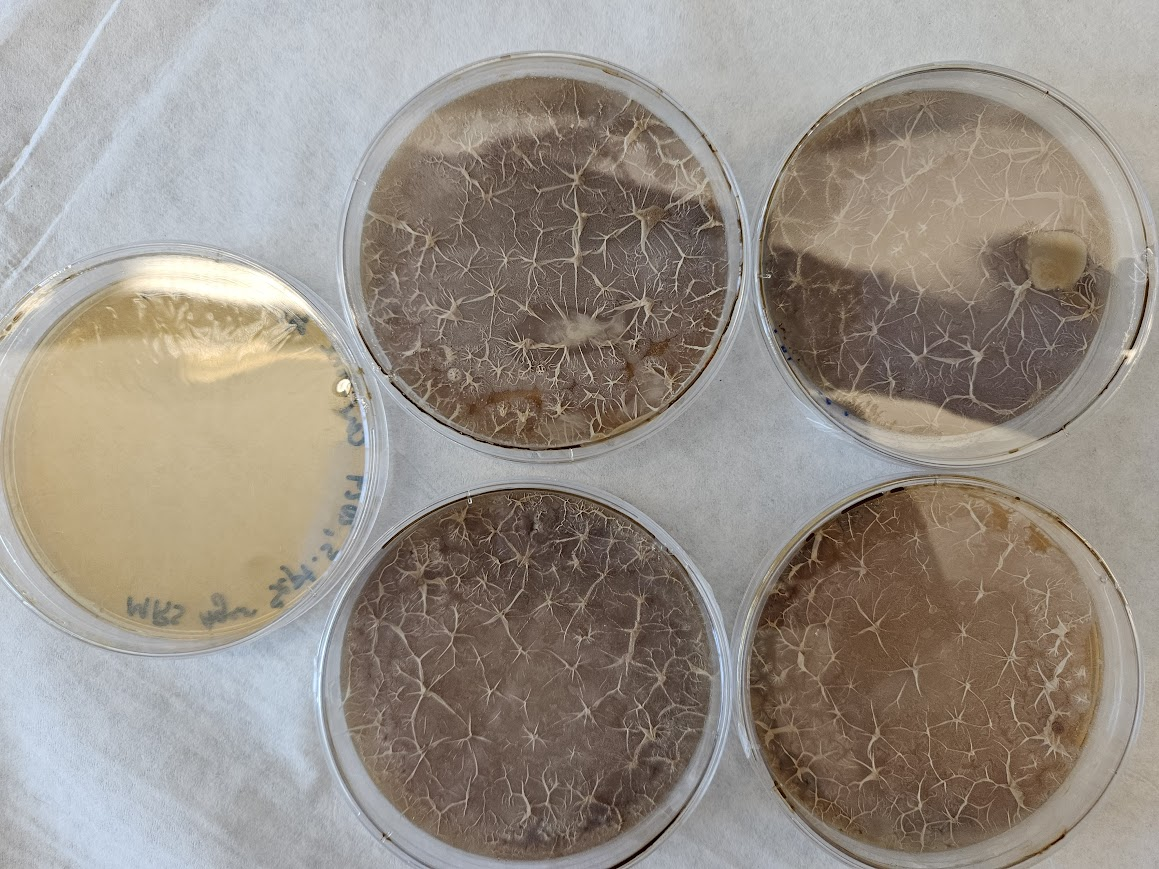
\includegraphics[width=0.85\textwidth]{Images/bacteria.png}
    \label{fig:bacteria_viability}
\end{figure}


\newpage
\section*{Appendix B}

% Change the figure labeling format for this appendix
\renewcommand{\thefigure}{B.\arabic{figure}}
\setcounter{figure}{0}  % Reset the figure counter

\begin{figure}[H]
    \captionsetup{justification=raggedright, singlelinecheck=false, position=above}  % Caption on top and left-justified
    \caption{Ethanol Standard Curves from Quartz Cuvette.}
    \centering
    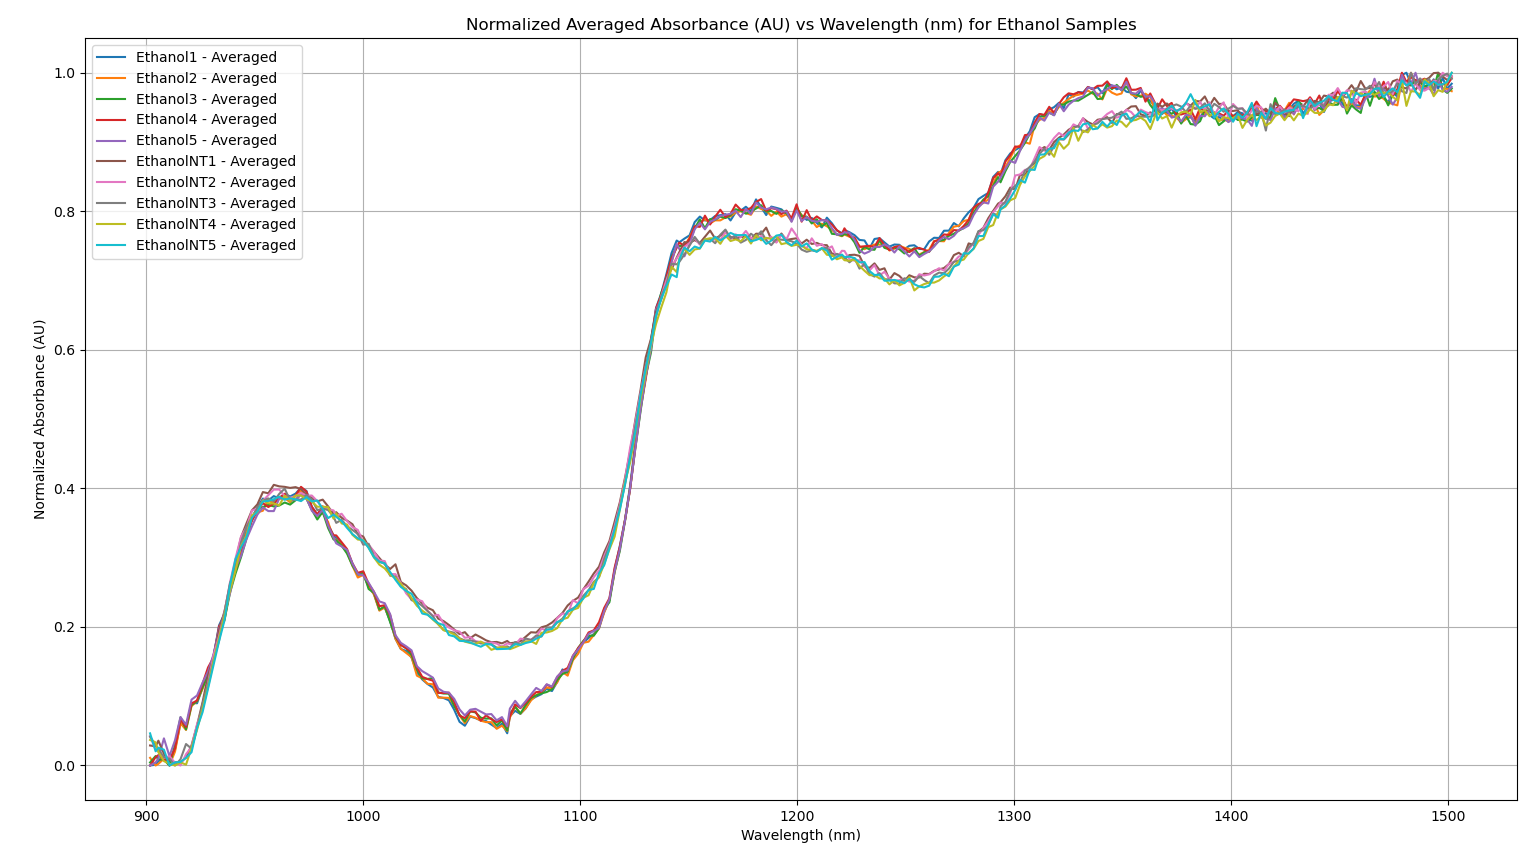
\includegraphics[width=\textwidth]{Images/Ethanol_Standard_Compared.png}
    \label{fig:appendix_ethanol_standard}
\end{figure}

\newpage
\begin{figure}[h]
  \captionsetup{justification=raggedright, singlelinecheck=false, position=above}  % Caption on top and left-justified
  \caption{Ethanol Standard Curve from Quartz vs Plastic Cuvette.}
  \centering
  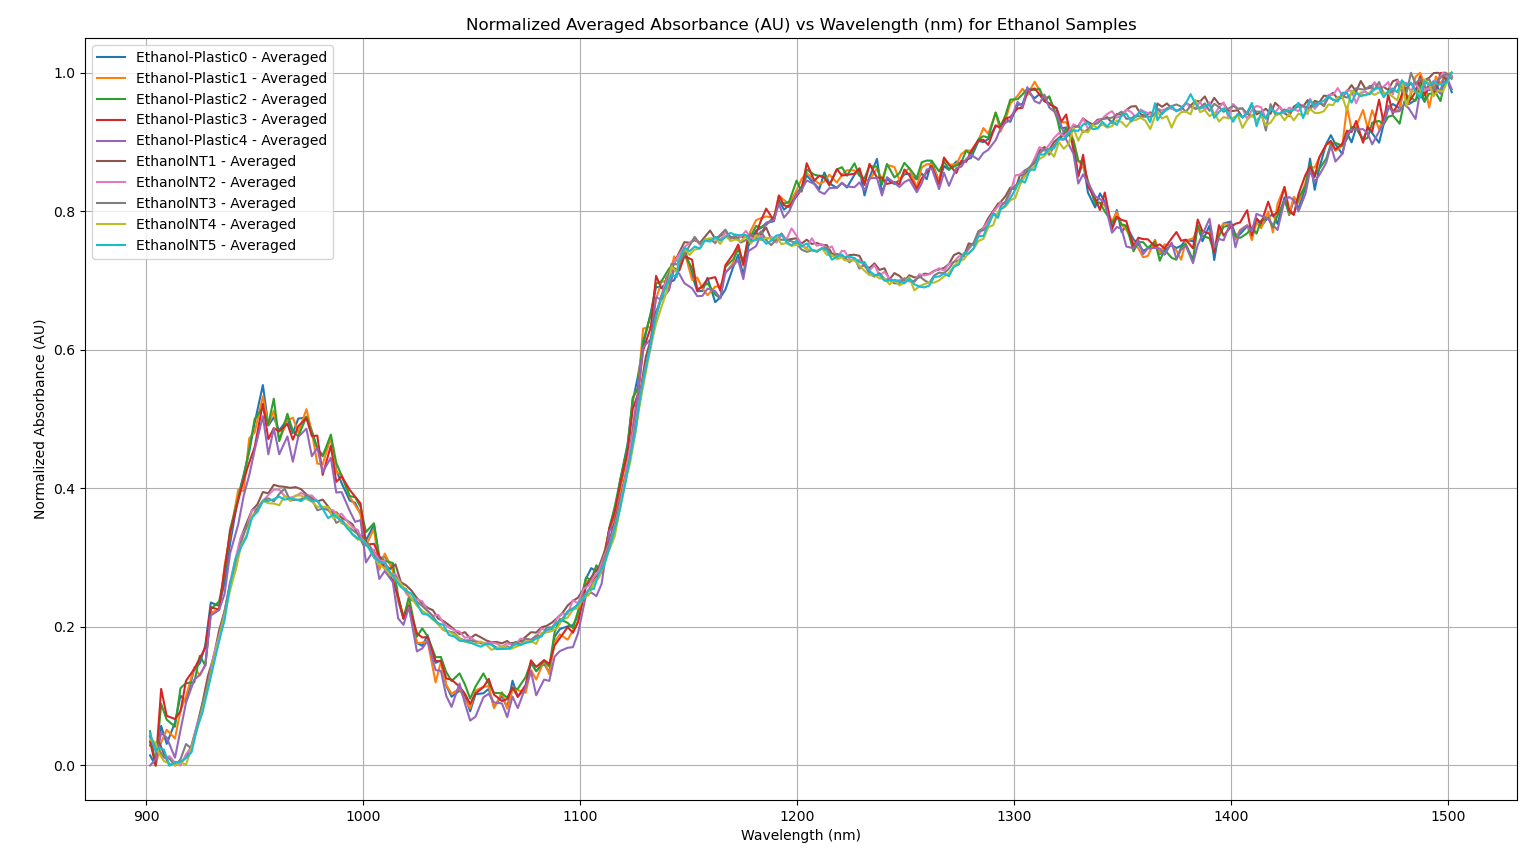
\includegraphics[width=\textwidth]{Images/Ethanol_Standard_PvQ.png}  % Replace with your image file
  \label{fig:appendix_ethanol_plastic}
\end{figure}

\newpage
\section*{Appendix C: Student Involvement}

\subsection*{Document}
\begin{itemize}
    \item \LaTeX - Connor
\end{itemize}

\subsection*{Materials \& Methods}
\begin{itemize}
    \item L. rhamnosus Viability Test - Shiza
    \item NIR Housing - Teflon component - Connor
    \item Quartz cuvette - Shiza
    \item Ethanol Standard Curve - Benji
    \item Data preprocessing: - Connor
    \item CNN Changes - Paola   
\end{itemize}

\subsection*{Results}
\begin{itemize}
    \item L. rhamnosus Viability Test - Shiza
    \item Ethanol standard curve comparison - Benji
    \item CNN Changes - Paola   
\end{itemize}

\subsection*{Discussion}
\begin{itemize}
    \item L. rhamnosus Viability Test - Shiza
    \item Ethanol curve - Benji
    \item CNN - Paola \& Connor
    \item Problems - Shiza
\end{itemize}

\subsection*{Future Steps}
\begin{itemize}
    \item L. rhamnosus Viability Test - Shiza
    \item Testing Fermentation - UV/Vis - Benji
    \item Data augmentation: gaussian noise and others - Connor
    \item Test with contamination - Paola
    \item Use new data to train the model (still being obtained) - Paola
\end{itemize}

\subsection*{Conclusion}
\begin{itemize}
    \item Conclusion - Everyone
\end{itemize}

% End document
\end{document}
